\documentclass[a4paper,14pt]{article}
\usepackage[utf8]{inputenc}
\usepackage[russian]{babel} 
\usepackage{graphicx} 
\usepackage{amsmath}
\usepackage{amssymb}
\usepackage{siunitx}% Для погрешностей
\usepackage{float}
\usepackage[colorlinks=true, linkcolor=blue]{hyperref}
\usepackage{enumitem}
\usepackage{longtable}
%\documentclass[fleqn]{article}

\renewcommand{\floatpagefraction}{0.99}
\renewcommand{\topfraction}{0.99}      



\title{ ЛАБОРАТОРНАЯ РАБОТА №2.2.

Основы измерений в цепях переменного тока}


\author{Батанин Артём Александрович}
\date{\today}


\begin{document}

\maketitle

\newpage
\tableofcontents    
\newpage            



\section{Цель работы}
Цель работы – познакомиться с принципом действия цифровых измерительных приборов; научиться проводить измерения в цепях переменного тока, определить рабочий диапазон по частоте различных цифровых мультиметров, провести измерение величины напряжения сигналов сложной формы и определить режимы работы источника гармонических сигналов.

\section{Оборудование}
Оборудование: генератор гармонических сигналов типа GFG, цифровые мультиметры типа GDM-8145, DT838 (или аналогичный), осциллограф, диод, макетные платы, тройник-разветвитель.

\section{Задание 1. Определение рабочего интервала частоты вольтметров}

Оборудование: Оборудование: генератор GFG 8255; вольтметры – цифровые
мультиметры GDM-8145 и DT838, разветвитель – тройник.

\begin{figure}[h!]
\centering
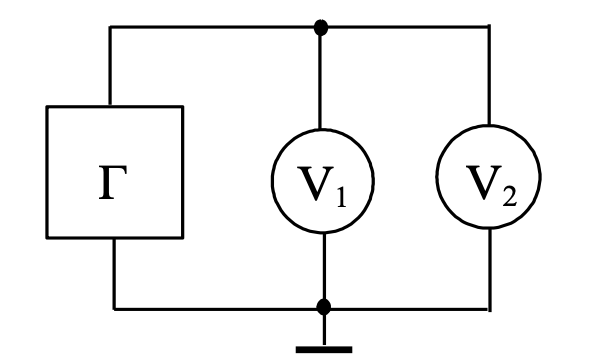
\includegraphics[width=0.5\linewidth]{schema1.png}
\caption{Схема для получения частотной харакеристики вольтметров:
Г – генератор гармонических колебаний GFG; V1 – цифровой
мультиметр GDM-8145; V2 – цифровой мультиметр DT838}
\label{fig:schema1}

\end{figure}

Измеренные значения представлены в \autoref{tab:tab1}, ниже приведен график (Рис. \ref{fig:gr0})

На основе измерений были получены рабочие диаппазоны (отклонение не более 10\% от максимально измеренного напряжения).

Для GDM рабочий диапазон: до 90 кГц (паспортный 50кГц);

Для DT838 рабочий диапазон: до 10 кГц (паспортный 400Гц).




\begin{figure}[H]
\centering
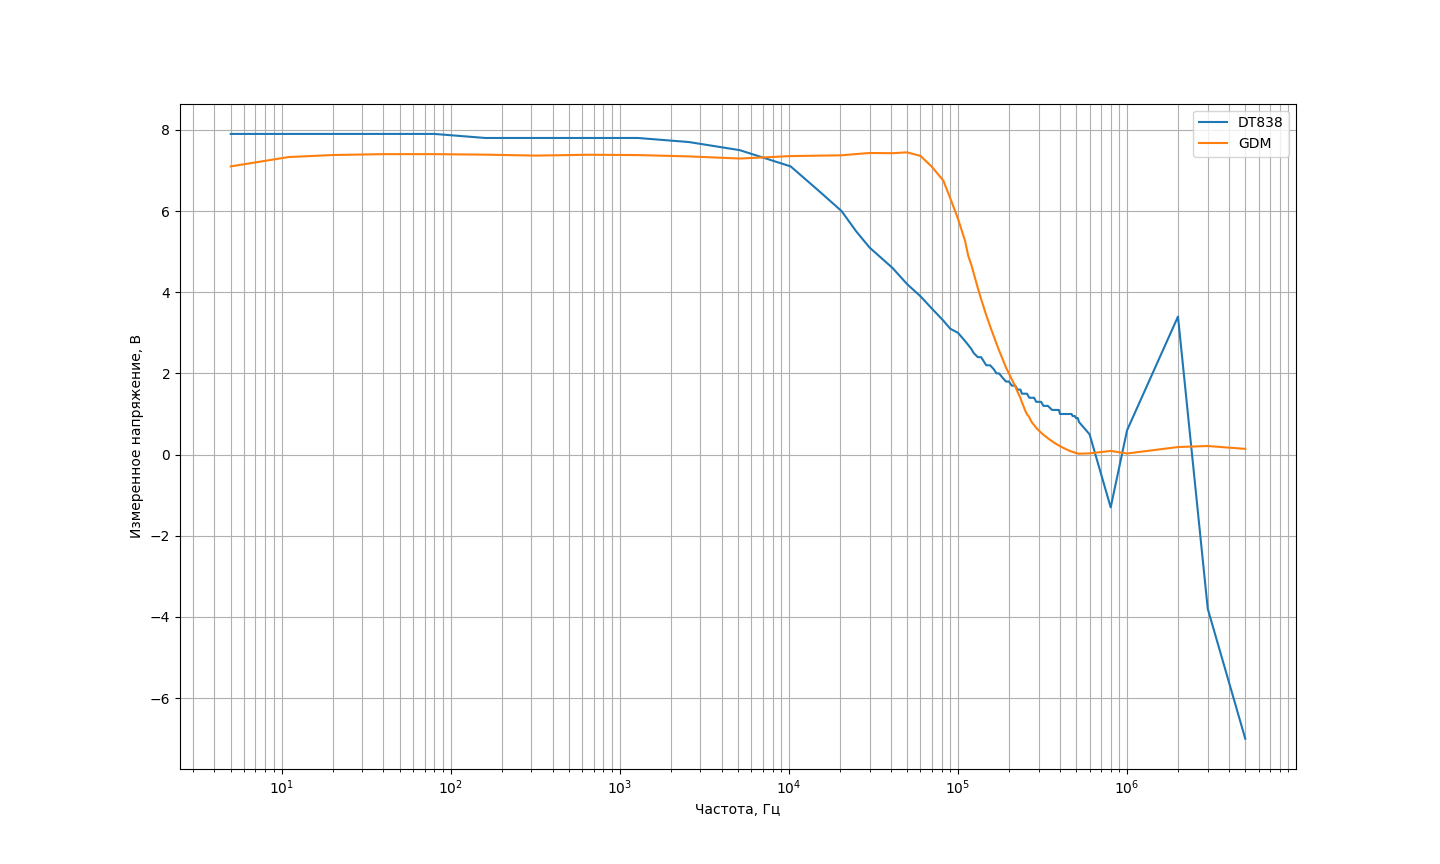
\includegraphics[width=1\linewidth]{gr1.png}
\caption{Зависимость измеренного напряжение вольтметрами GDM и DT838}
\label{fig:gr0}

\end{figure}







\section {Задание 2. Изучение влияния амперметра на режим
работы электрической цепи постоянного тока}
Оборудование: генератор GFG; осциллограф Tektronix; вольтметр – цифровой мультиметр GDM-8145; разветвитель-тройник.



\begin{figure}[h!]
\centering
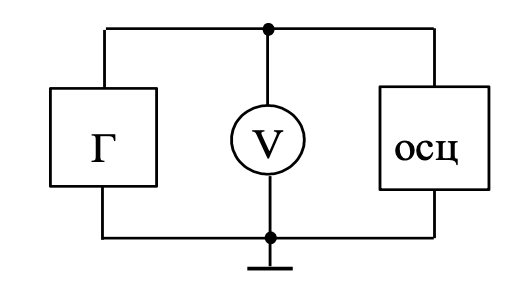
\includegraphics[width=0.5\linewidth]{schema2.png}
\caption{Измерение периодических сигналов:
Г – генератор GFG; V – цифровой мультиметр
GDM-8145; ОСЦ – осциллограф Tektronix}
\label{fig:schema2}

\end{figure}


\begin{table}[htbp]
  \centering
  \caption{Таблица к заданию 2}
  \label{tab:tab2}
  \begin{tabular}{|c|c|c|c|c|c|}
    \hline
    Форма сигнала  & GDM AC true RMS, В & $\Delta U_{\text{GDM}}$ & Рассчетные & Tektronix (PK-PK), В &  $\Delta U_{\text{Осц}}$    \\ \hline
    Синус  & 7.294 & 0.01& 10.3 & 10.5 & 0.08  \\ \hline
    Треугольный  & 6.379 & 0.01& 11.08 & 10.8 & 0.08  \\ \hline
    Прямоугольный  & 11.29 & 0.01& 11.29 & 10.9 & 0.08  \\ \hline
  \end{tabular}
\end{table}

%form pkpk gdm
%sine 10.5 7.294
%triangle 10.8 6.397
%meandr 10.9 11.29

\section{Задание 3. Измерение напряжения периодических сигналов с постоянной составляющей}

\subsection{Рассчет теоретических значений для треугольного сигнала}

\begin{equation}
\begin{aligned}
\hat{U}  = \frac{2}{T}\int_{0}^{T/4}{4\frac{U_{pkpk} t dt }{T}}\\
\hat{U}  = \frac{8U_{pkpk}}{T^2}\int_{0}^{T/4}{ t dt}\\
\hat{U}  = \frac{8U_{pkpk} \cdot T^2 }{T^2 \cdot 32}\\
\hat{U} = \frac{U_{pkpk}}{4} \text{Среднее напряжение (DC)}
\label{exp}
 \end{aligned}
\end{equation}


\begin{equation}
\begin{aligned}
U_{RMS}  =  \sqrt{\frac{2}{T}\int_{0}^{T/4}{(4\frac{U_{pkpk} t  }{T})^2} dt}\\
U_{RMS}  =  \sqrt{\frac{U_{pkpk}^2 32}{T^3}\int_{0}^{T/4}{t^2}dt}\\
U_{RMS}  =  \sqrt{\frac{U_{pkpk}^2 32 \cdot T^3}{T^3 \cdot 3 \cdot 64}}\\
U_{RMS}  =  \frac{U_{pkpk}}{\sqrt{6}} \text{Действующее напряжение (RMS)}
 \label{exp}
 \end{aligned}
\end{equation}



\subsection{Рассчет теоретических значений для прямоугольного сигнала}

\begin{equation}
\begin{aligned}
\hat{U}  = \frac{1}{T}\int_{0}^{T/2}{U_{pkpk} dt }\\
\hat{U}  = \frac{U_{pkpk}}{T}\int_{0}^{T/2}{ t dt}\\
\hat{U}  = \frac{U_{pkpk}\cdot T}{T\cdot 2}\\
\hat{U} = \frac{U_{pkpk}}{2} \text{Среднее напряжение (DC)}
\label{exp}
 \end{aligned}
\end{equation}


\begin{equation}
\begin{aligned}
U_{RMS}  =  \sqrt{ \frac{1}{T}\int_{0}^{T/2}{U_{pkpk}^2 dt }}\\
U_{RMS}  =  \frac{U_{pkpk}}{\sqrt{2}} \text{Действующее напряжение (RMS)}
 \label{exp}
 \end{aligned}
\end{equation}

\subsection{Эксперимент}

Ниже приведена таблица с измеренными значениями и с расчетными значениями (\autoref{tab:tab3})

\begin{figure}[H]
\centering
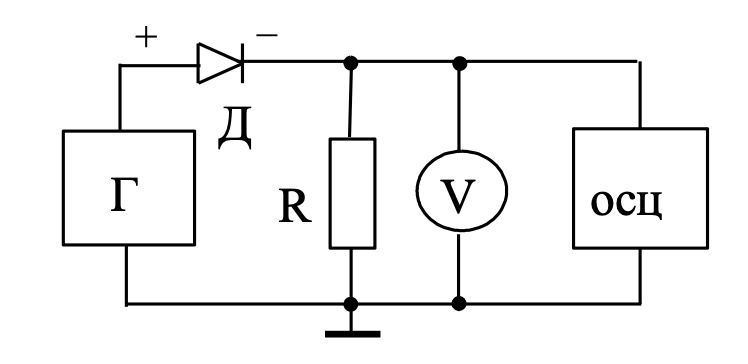
\includegraphics[width=0.5\linewidth]{schema3.png}
\caption{Измерение сигналов сложной формы:
Г – генератор GFG; ОСЦ – осциллограф Tektronix;
V – цифровой мультиметр GDM-8145; Д – полупроводниковый диод; R – сопротивление 1 кОм}
\label{fig:schema3}

\end{figure}



\begin{table}[htbp]
  \centering
  \caption{Таблица к заданию 2}
  \label{tab:tab3}
  \begin{tabular}{|c|c|c|c|c|c|}
    \hline
    Форма  & GDM AC true RMS, В & GDM DC, В & $DC_{\text{расч}}$ & $AC_{\text{расч}}$ &PK-PK, В     \\ \hline
    Синус  & \num{3.005\pm 0.01}& \num{4.75\pm 0.01} & 9.44 & 9.5 & \num{9.76\pm 0.08}  \\ \hline
    Треугольный  & \num{2.45\pm 0.01} & \num{4.089\pm 0.01}& 9.8 & 10.02 & \num{10.2\pm 0.08}  \\ \hline
    Прямоугольный  & \num{5.54\pm 0.01} & \num{7.191\pm 0.01}& 11.08 & 10.16 & \num{10.2\pm 0.08}  \\ \hline
  \end{tabular}
\end{table}


%sine 3.005  4.75  9.76
%triangle 2.45 4.089 10.2
%meandr 5.54 7.191 10.2





\section{Задание 4. Изучение зависимости мощности, выделяемой на нагрузке, от соотношения сопротивления источника и сопротивления нагрузки}

\begin{figure}[H]
\centering
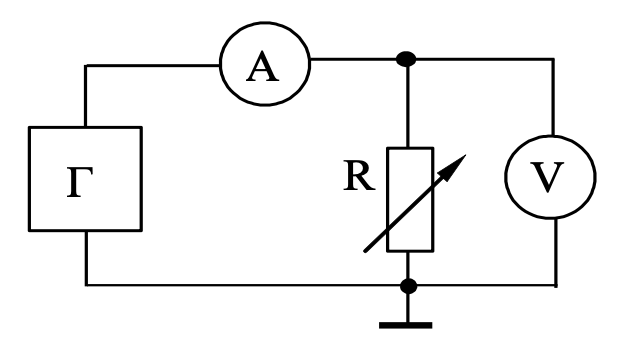
\includegraphics[width=0.5\linewidth]{schema4.png}
\caption{Схема установки для изучения режима работы
генератора: Г – источник гармонических сигналов GFG;
А – амперметр – мультиметр GDM-8145; V – вольтметр
– мультиметр GDM-8145; R – магазин сопротивлений}
\label{fig:schema4}
\end{figure}





\begin{table}[htbp]
  \centering
  \caption{Таблица к заданию 4}
  \label{tab:tab4}
  \begin{tabular}{|c|c|c|c|}
    \hline
    Сопротивление, Ом & Напряжение, В & Ток, мА & Мощность, Вт   \\ \hline
99.9 & \num{4.686 \pm 0.01} & \num{46.85 \pm 0.06} & 0.22   \\ \hline
89.9 & \num{4.506 \pm 0.01} & \num{50.08 \pm 0.06} & 0.226   \\ \hline
79.9 & \num{4.305 \pm 0.01} & \num{53.78 \pm 0.06} & 0.232   \\ \hline
69.9 & \num{4.079 \pm 0.01} & \num{58.34 \pm 0.06} & 0.238   \\ \hline
59.9 & \num{3.811 \pm 0.01} & \num{63.44 \pm 0.06} & 0.242   \\ \hline
49.9 & \num{3.483 \pm 0.01} & \num{69.72 \pm 0.06} & 0.243   \\ \hline
39.9 & \num{3.086 \pm 0.01} & \num{77.49 \pm 0.06} & 0.239   \\ \hline
29.9 & \num{2.619 \pm 0.01} & \num{87.59 \pm 0.06} & 0.229   \\ \hline
19.9 & \num{1.84 \pm 0.01} & \num{94.0 \pm 0.06} & 0.173   \\ \hline
9.9 & \num{1.086 \pm 0.01} & \num{111.0 \pm 0.06} & 0.121   \\ \hline


  \end{tabular}
\end{table}



\begin{figure}[H]
\centering
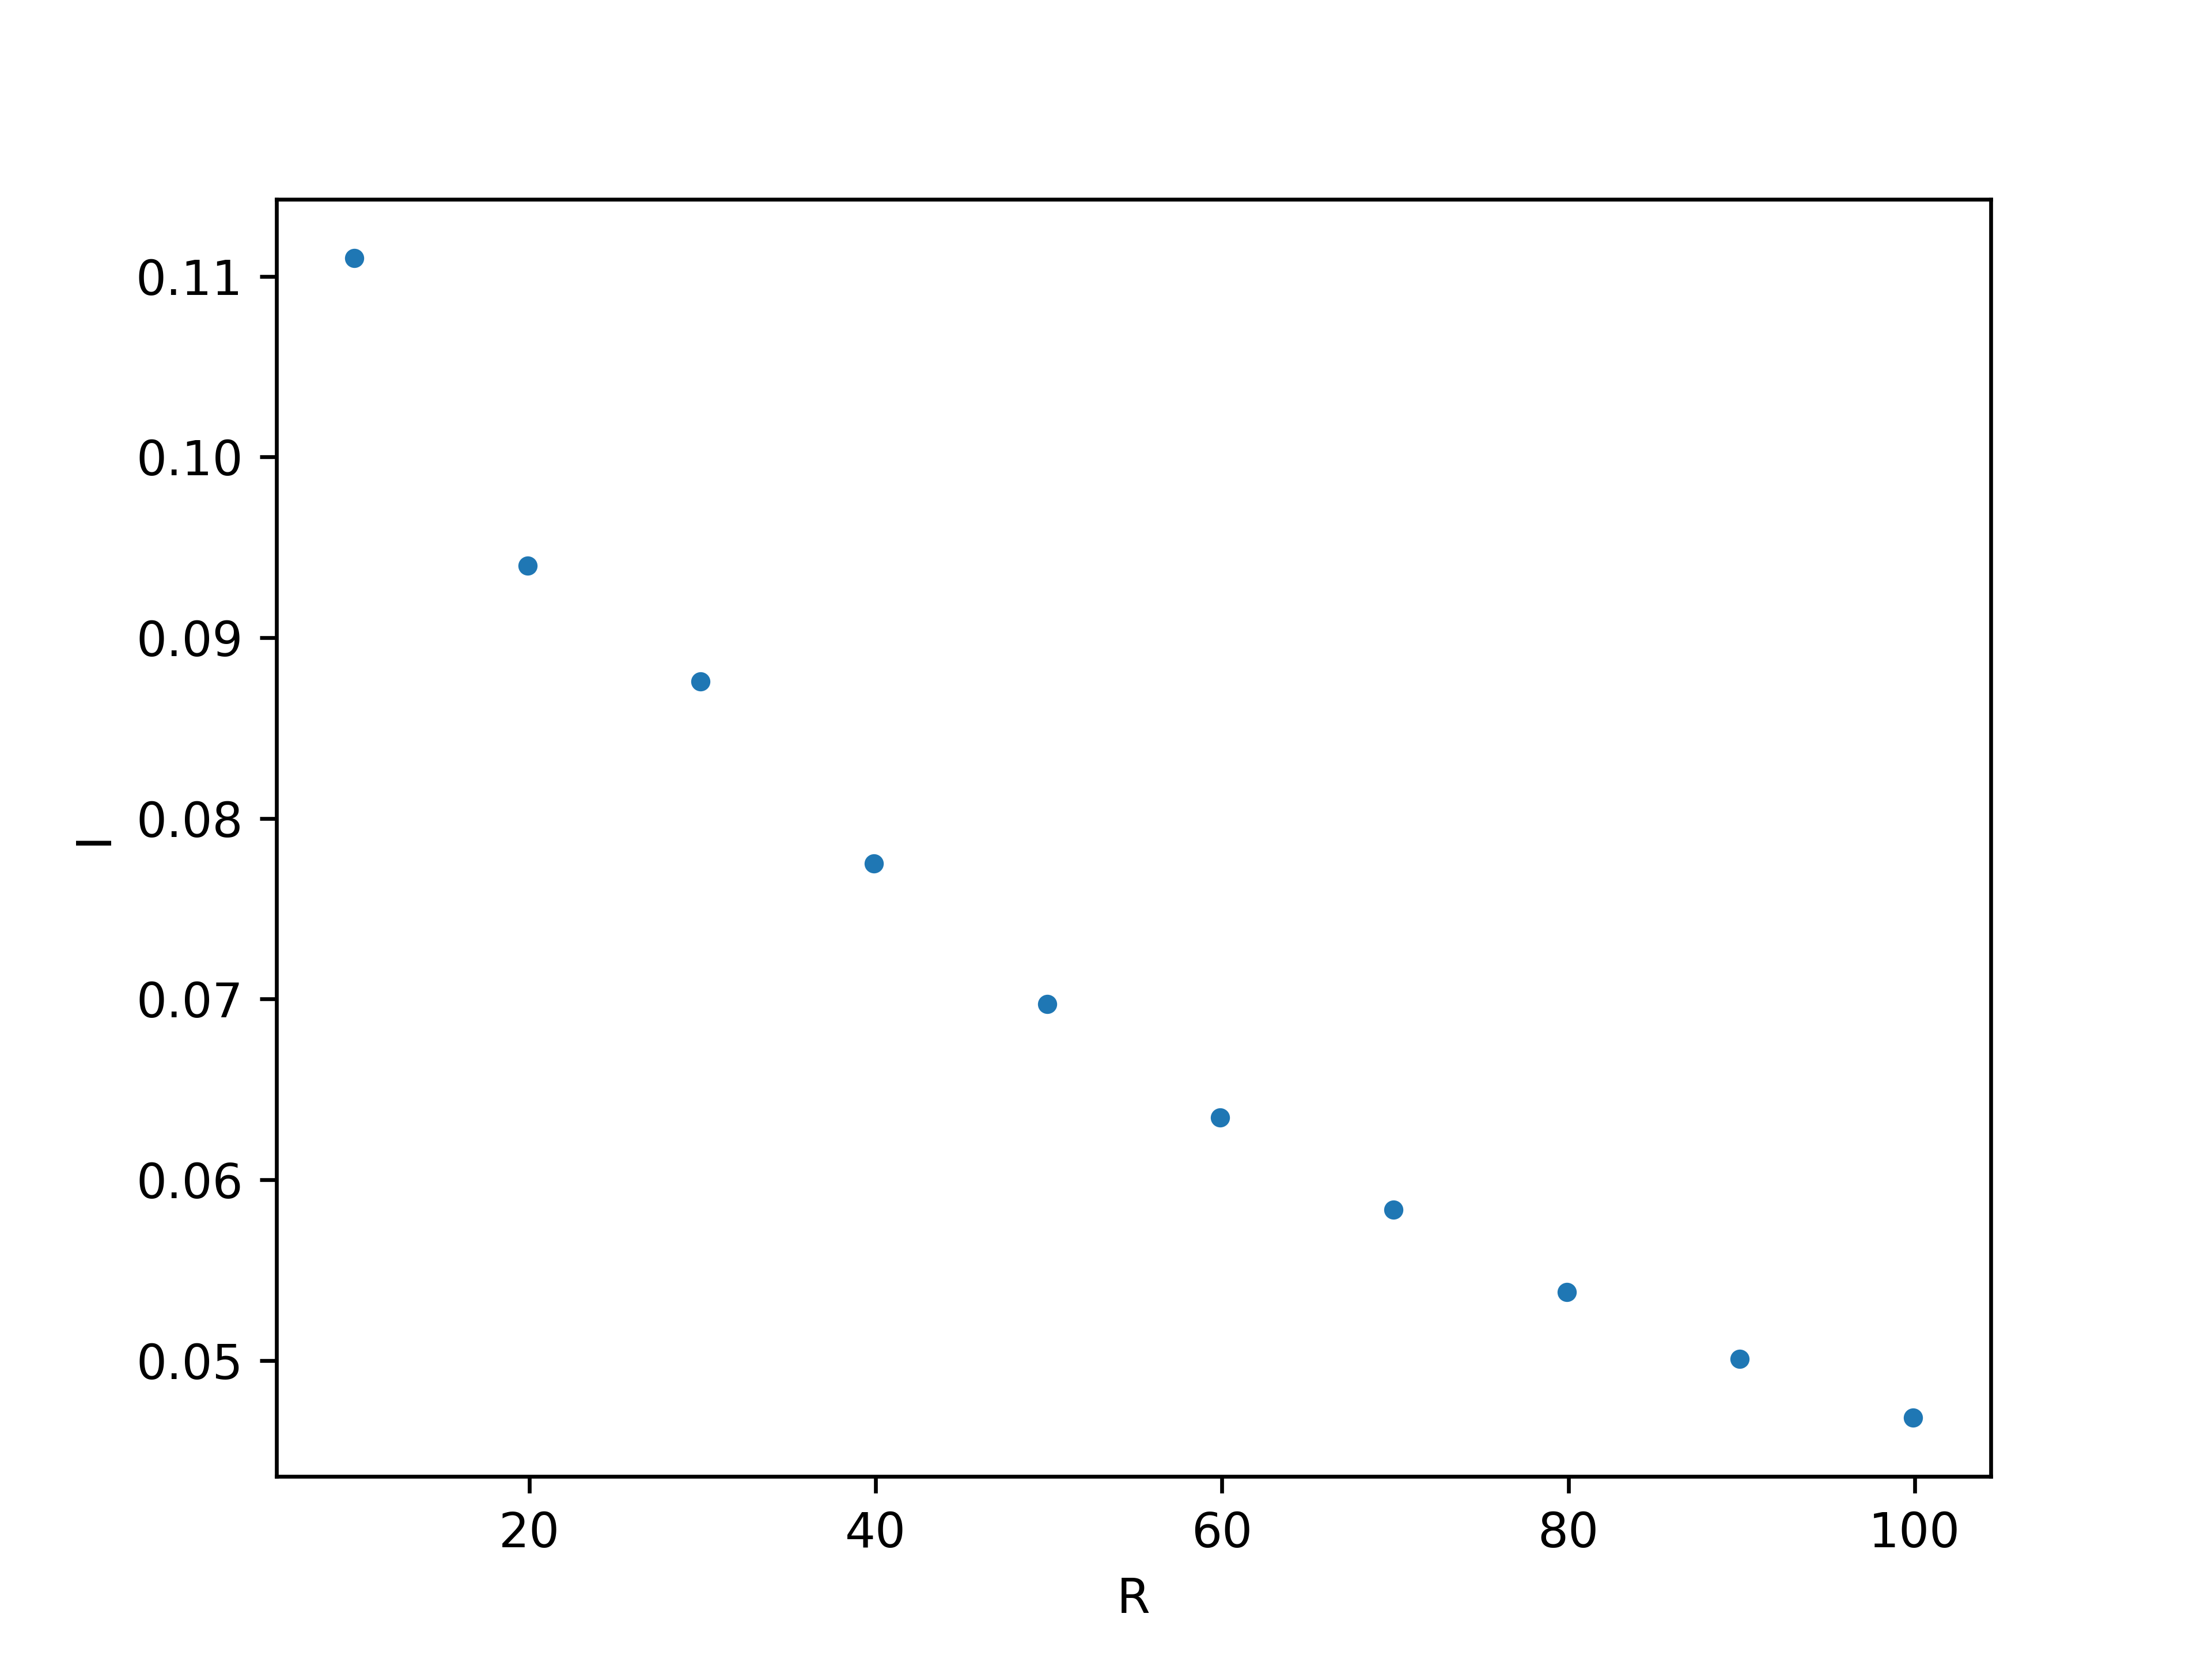
\includegraphics[width=1\linewidth]{R_I.png}
\caption{Зависимость силы тока от сопротивления}
\label{fig:R_I}
\end{figure}

\begin{figure}[H]
\centering
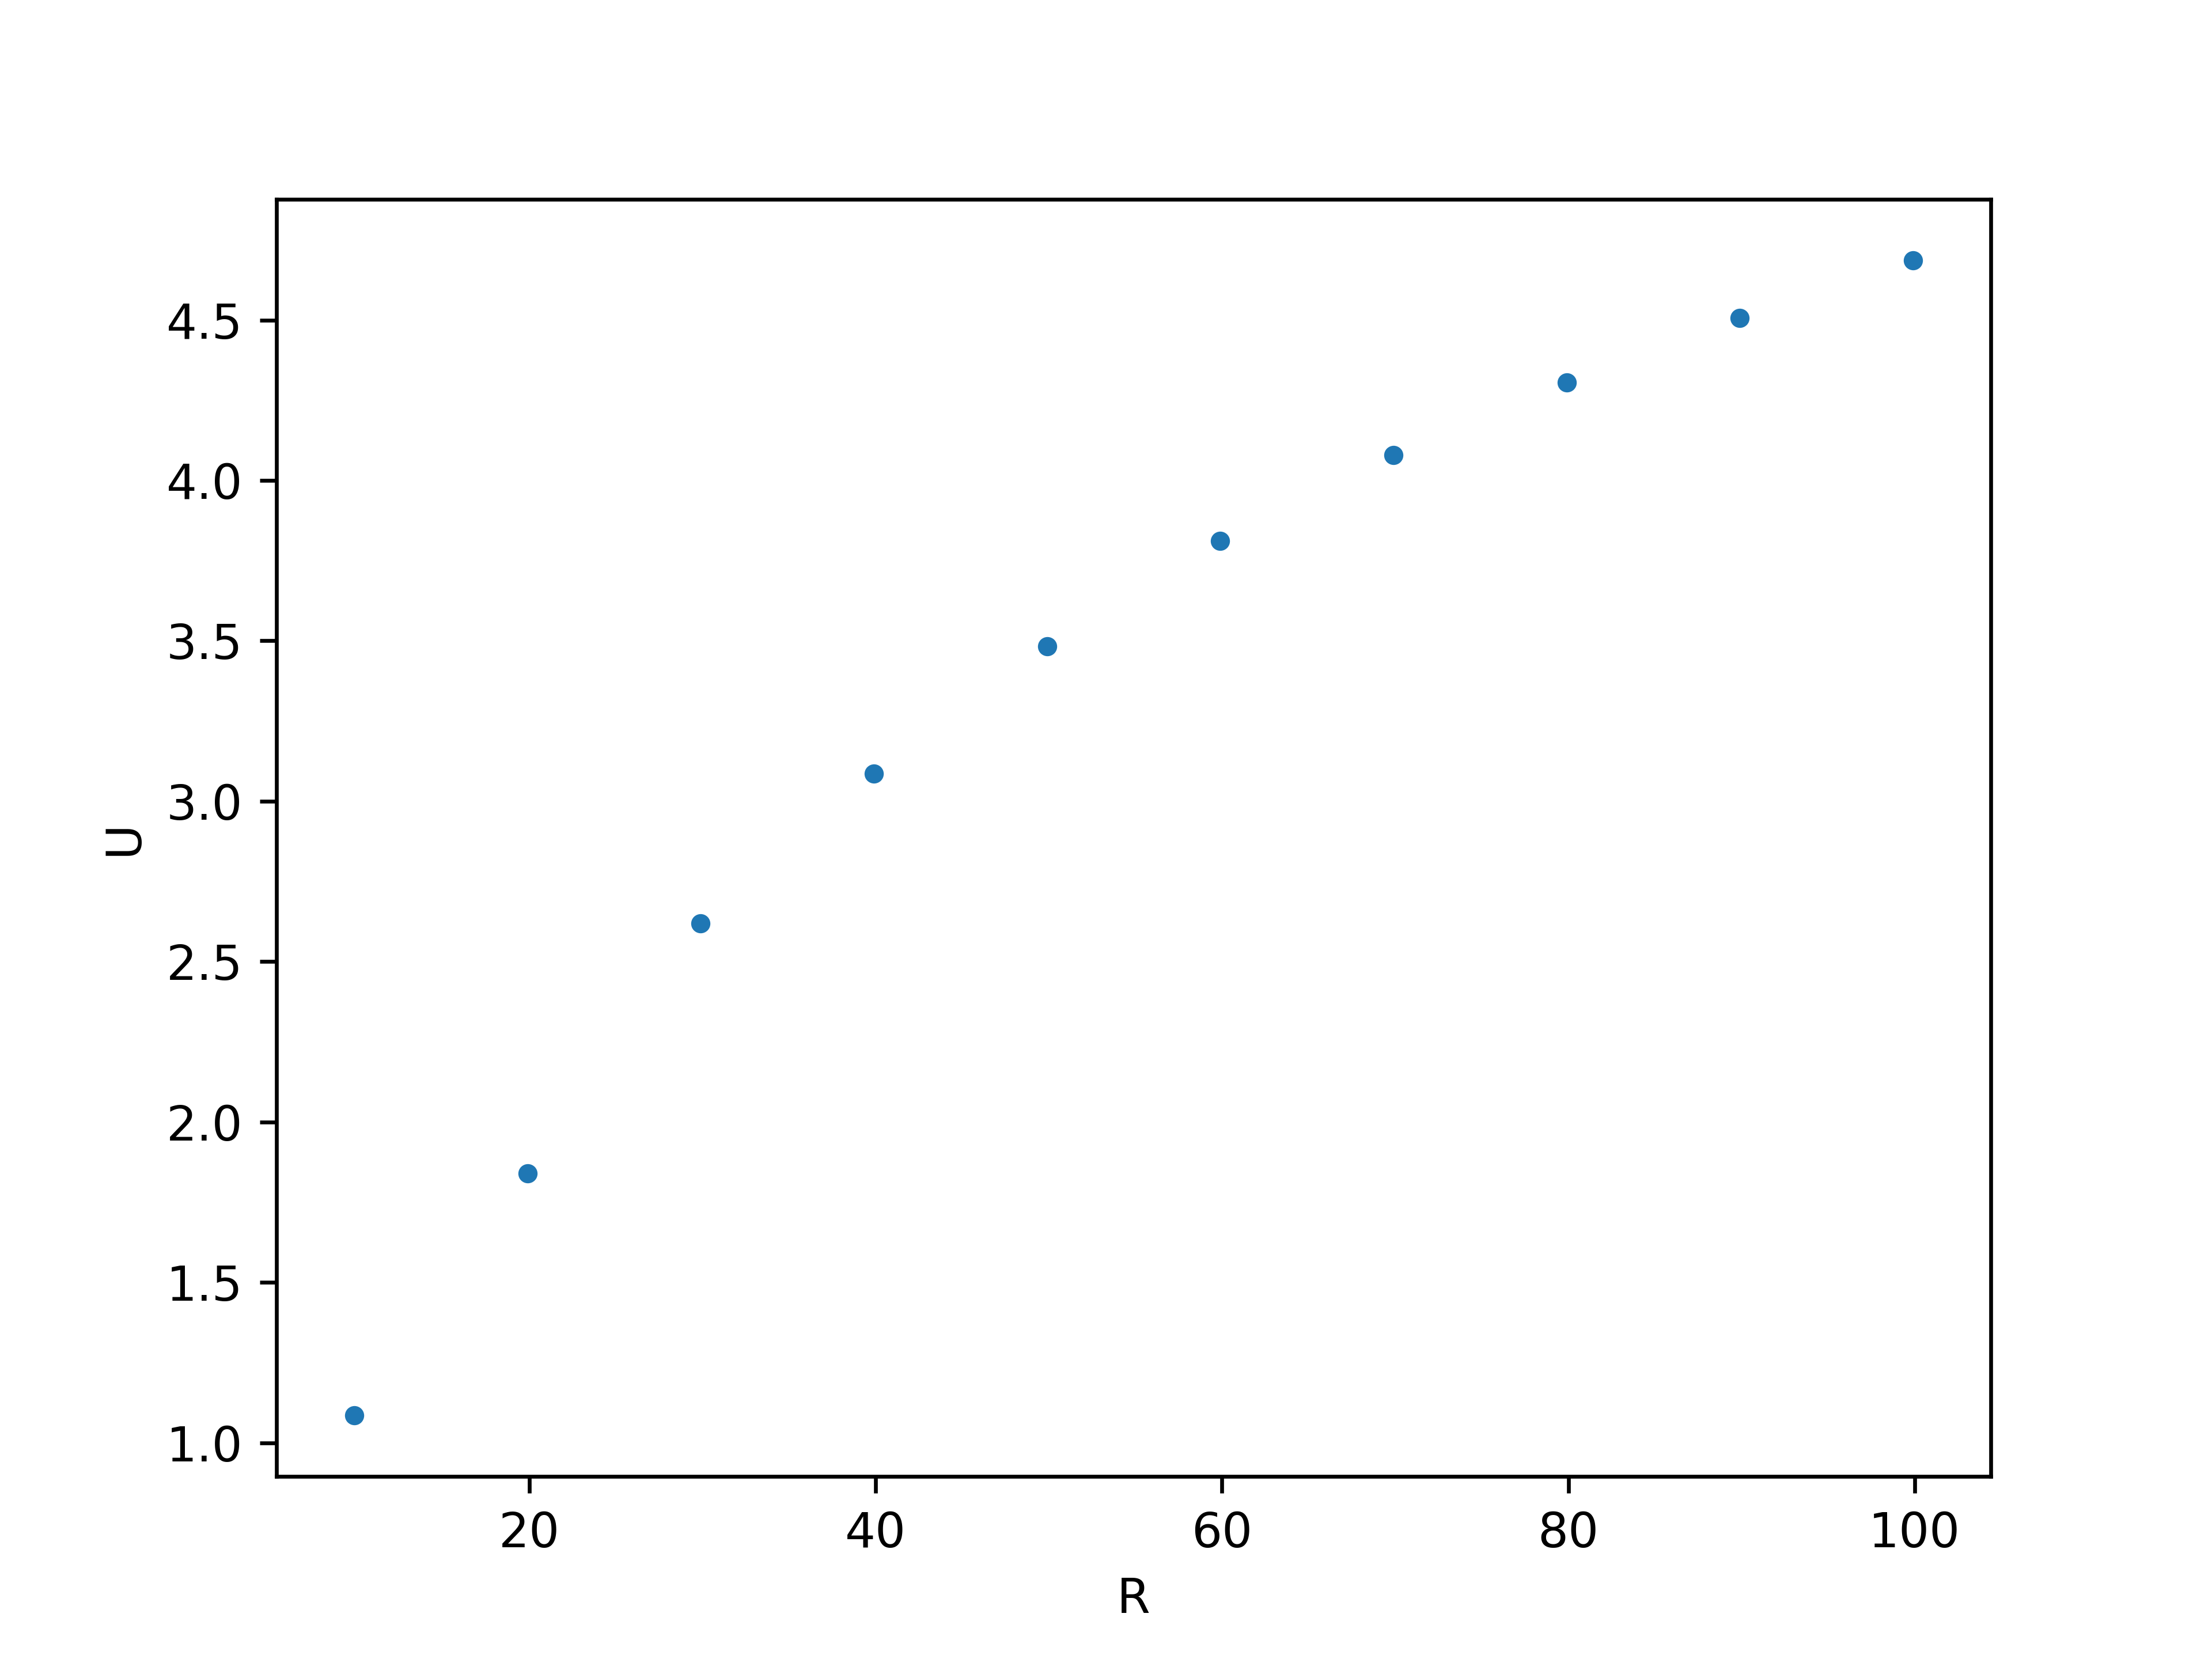
\includegraphics[width=1\linewidth]{R_U.png}
\caption{Напряжения от сопротивления}
\label{fig:R_I}
\end{figure}

\begin{figure}[H]
\centering
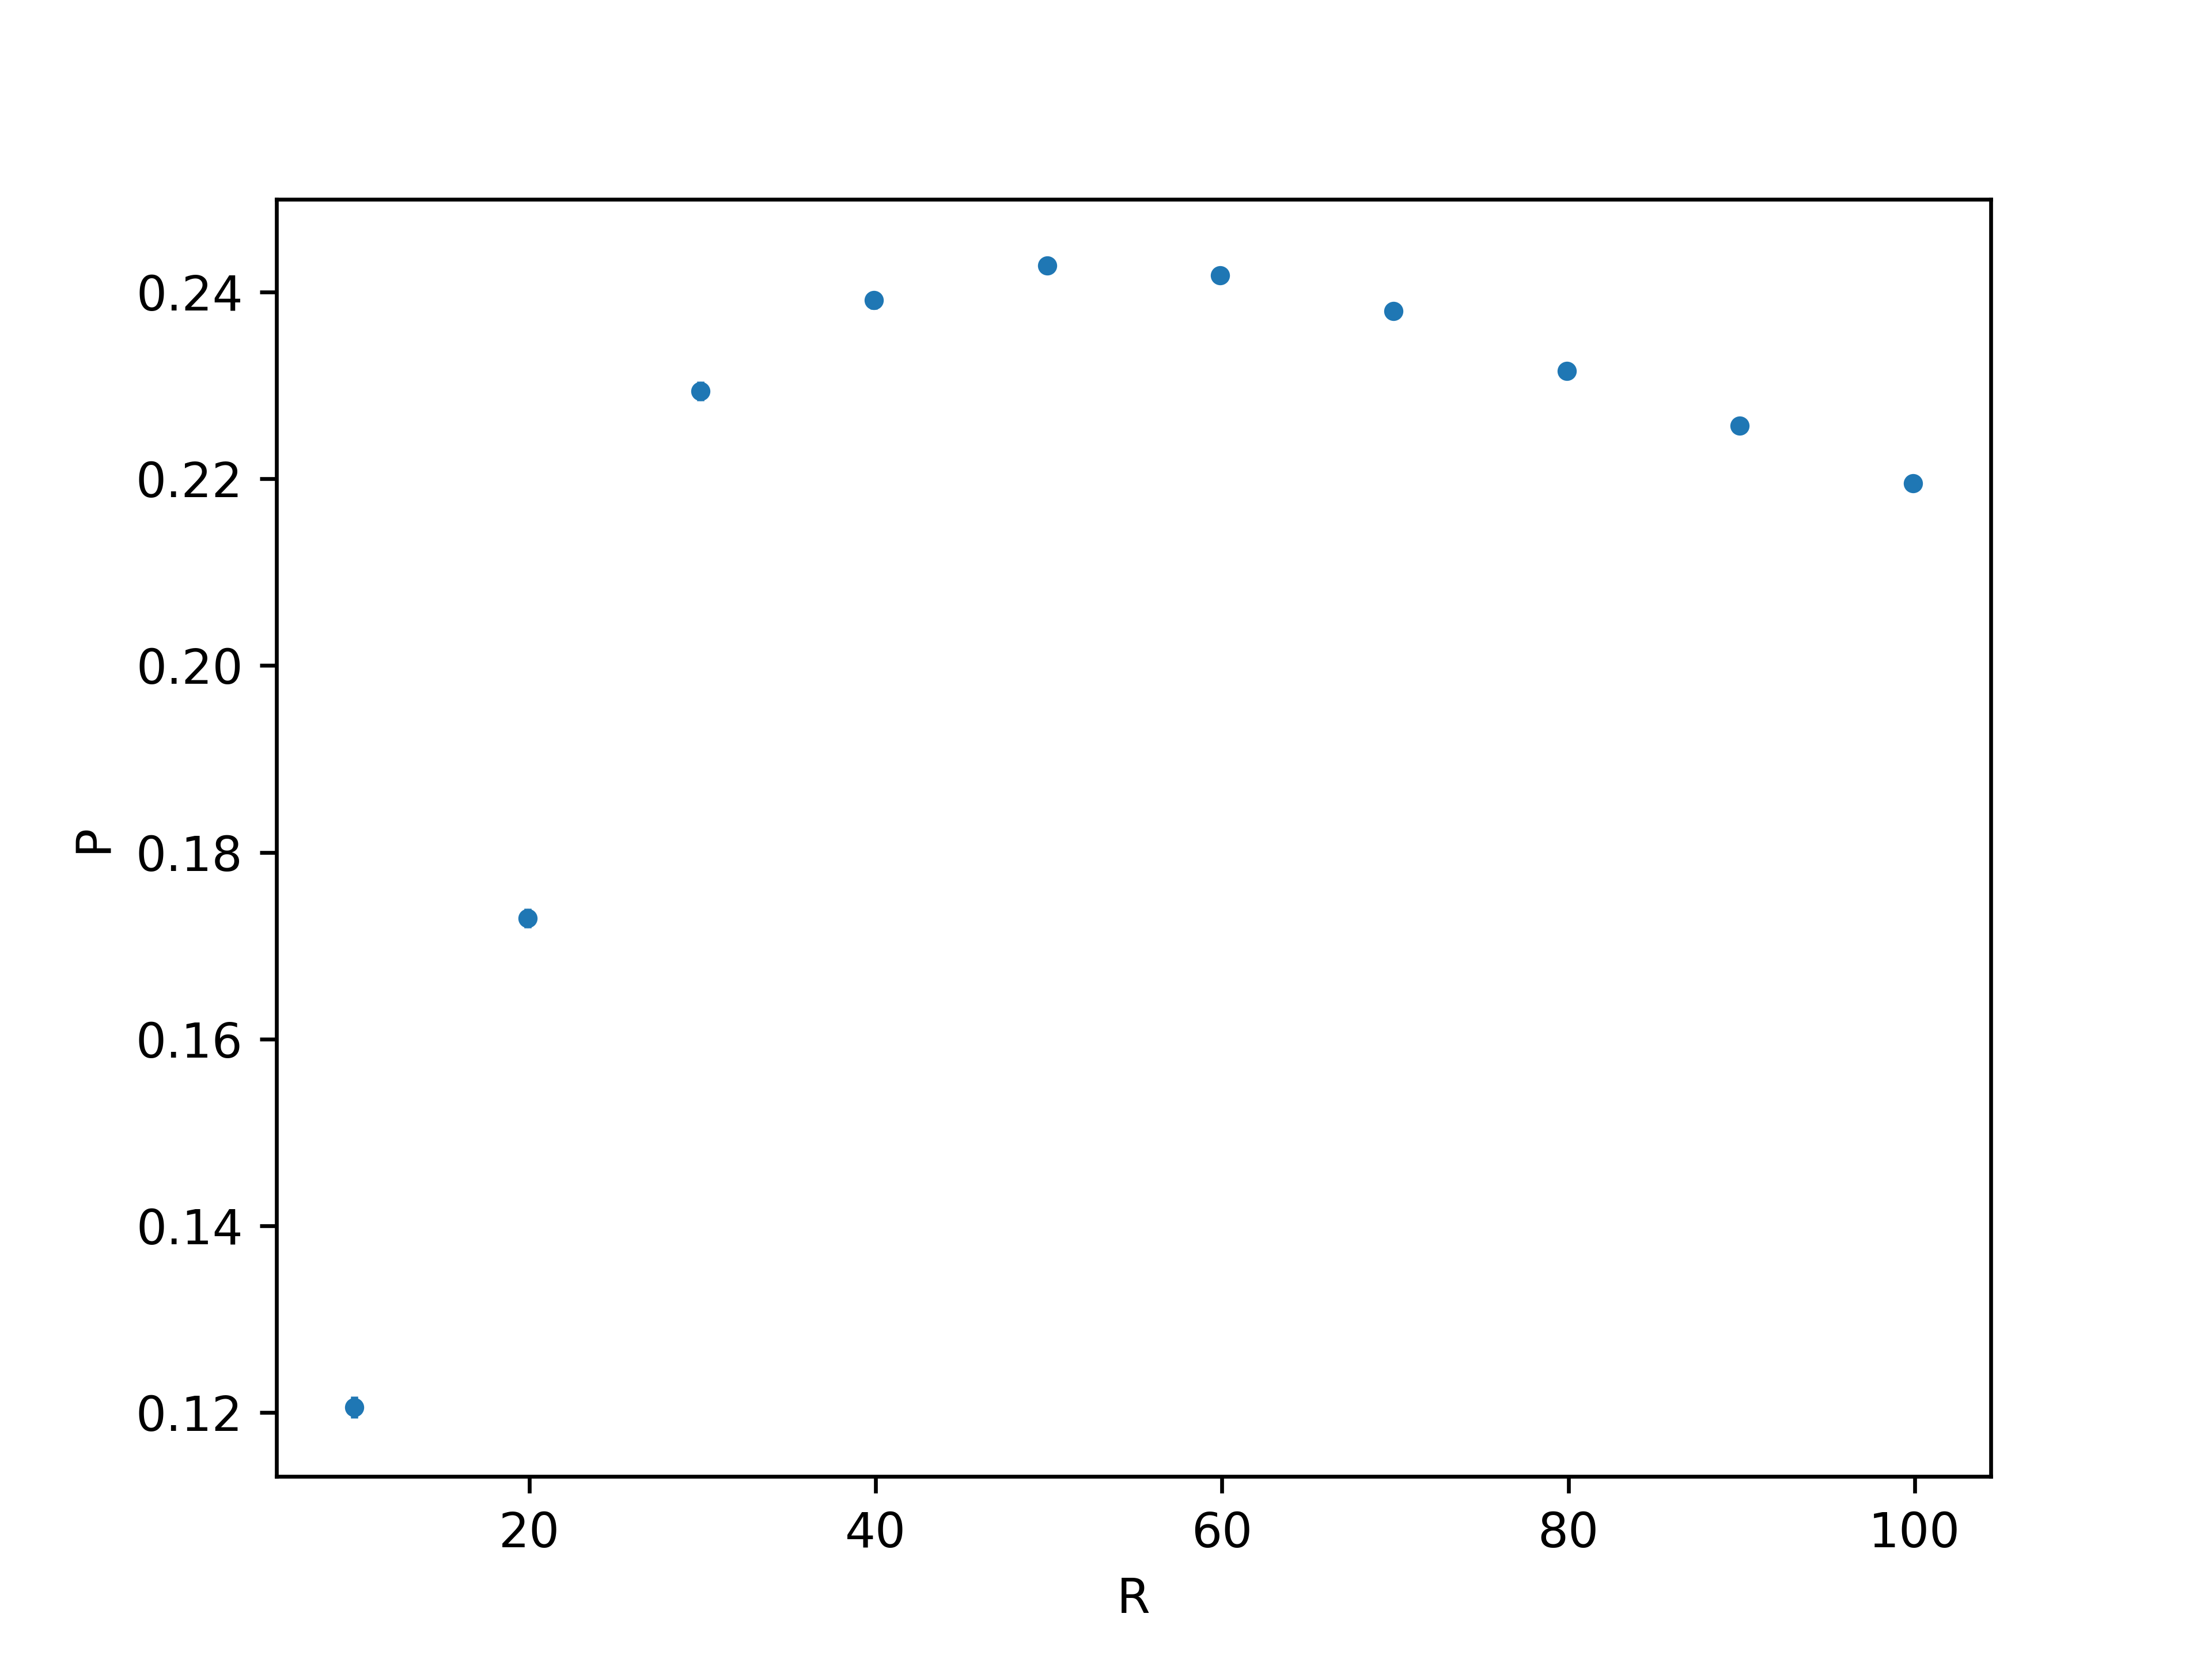
\includegraphics[width=1\linewidth]{R_P.png}
\caption{Мощности от сопротивления}
\label{fig:R_I}
\end{figure}

На основе данных были получены значения ЭДС источника и его внутреннее сопротивление:
$E = 7.3$ В

$r = \num{55 \pm 0.2}$ Ом


\section{Результаты измерений}


\begin{longtable}{|c|c|c|}
    % 1. Шапка на САМОЙ ПЕРВОЙ странице
    \caption{Таблица к заданию 1} \label{tab:tab1} \\
    \hline
    \textbf{Частота, Гц} & \textbf{GDM, В} & \textbf{DT838, В} \\
    \hline
    \endfirsthead

    % 2. Шапка на ВСЕХ ПОСЛЕДУЮЩИХ страницах
    \hline
    \textbf{Частота, Гц} & \textbf{GDM, В} & \textbf{DT838, В} \\
    \hline
    \endhead

    % 3. Подвал на ПРОМЕЖУТОЧНЫХ страницах (указывает на продолжение)
    \hline
    \multicolumn{3}{|c|}{\textit{Продолжение на следующей странице...}} \\
    \hline
    \endfoot

    % 4. Подвал на САМОЙ ПОСЛЕДНЕЙ странице таблицы
    \hline
    \endlastfoot

    % --- ТЕЛО ТАБЛИЦЫ (ваши данные) ---
5 & 7.1 & 7.9   \\ \hline
11 & 7.33 & 7.9   \\ \hline
20 & 7.38 & 7.9   \\ \hline
40 & 7.402 & 7.9   \\ \hline
80 & 7.402 & 7.9   \\ \hline
160 & 7.389 & 7.8   \\ \hline
320 & 7.366 & 7.8   \\ \hline
654 & 7.387 & 7.8   \\ \hline
1280 & 7.379 & 7.8   \\ \hline
2560 & 7.346 & 7.7   \\ \hline
5120 & 7.294 & 7.5   \\ \hline
$1.02 \cdot 10^4 $ & 7.354 & 7.1   \\ \hline
$1.5 \cdot 10^4 $ & 7.365 & 6.5   \\ \hline
$2.05 \cdot 10^4 $ & 7.373 & 6.0   \\ \hline
$2.5 \cdot 10^4 $ & 7.404 & 5.5   \\ \hline
$3.0 \cdot 10^4 $ & 7.43 & 5.1   \\ \hline
$4.1 \cdot 10^4 $ & 7.425 & 4.6   \\ \hline
$5.0 \cdot 10^4 $ & 7.446 & 4.2   \\ \hline
$6.0 \cdot 10^4 $ & 7.358 & 3.9   \\ \hline
$7.0 \cdot 10^4 $ & 7.093 & 3.6   \\ \hline
$8.19 \cdot 10^4 $ & 6.75 & 3.3   \\ \hline
$9.0 \cdot 10^4 $ & 6.315 & 3.1   \\ \hline
$1.0 \cdot 10^5 $ & 5.81 & 3.0   \\ \hline
$1.1 \cdot 10^5 $ & 5.269 & 2.8   \\ \hline
$1.15 \cdot 10^5 $ & 4.895 & 2.7   \\ \hline
$1.2 \cdot 10^5 $ & 4.669 & 2.6   \\ \hline
$1.24 \cdot 10^5 $ & 4.459 & 2.5   \\ \hline
$1.31 \cdot 10^5 $ & 4.103 & 2.4   \\ \hline
$1.37 \cdot 10^5 $ & 3.831 & 2.4   \\ \hline
$1.47 \cdot 10^5 $ & 3.432 & 2.2   \\ \hline
$1.55 \cdot 10^5 $ & 3.158 & 2.2   \\ \hline
$1.63 \cdot 10^5 $ & 2.909 & 2.1   \\ \hline
$1.69 \cdot 10^5 $ & 2.731 & 2.0   \\ \hline
$1.75 \cdot 10^5 $ & 2.564 & 2.0   \\ \hline
$1.83 \cdot 10^5 $ & 2.369 & 1.9   \\ \hline
$1.92 \cdot 10^5 $ & 2.15 & 1.8   \\ \hline
$2.0 \cdot 10^5 $ & 2.0 & 1.8   \\ \hline
$2.08 \cdot 10^5 $ & 1.852 & 1.7   \\ \hline
$2.18 \cdot 10^5 $ & 1.682 & 1.7   \\ \hline
$2.25 \cdot 10^5 $ & 1.548 & 1.6   \\ \hline
$2.34 \cdot 10^5 $ & 1.396 & 1.6   \\ \hline
$2.39 \cdot 10^5 $ & 1.284 & 1.5   \\ \hline
$2.45 \cdot 10^5 $ & 1.175 & 1.5   \\ \hline
$2.49 \cdot 10^5 $ & 1.095 & 1.5   \\ \hline
$2.56 \cdot 10^5 $ & 0.994 & 1.5   \\ \hline
$2.64 \cdot 10^5 $ & 0.922 & 1.4   \\ \hline
$2.7 \cdot 10^5 $ & 0.833 & 1.4   \\ \hline
$2.75 \cdot 10^5 $ & 0.782 & 1.4   \\ \hline
$2.82 \cdot 10^5 $ & 0.726 & 1.4   \\ \hline
$2.9 \cdot 10^5 $ & 0.66 & 1.3   \\ \hline
$3.0 \cdot 10^5 $ & 0.597 & 1.3   \\ \hline
$3.1 \cdot 10^5 $ & 0.54 & 1.3   \\ \hline
$3.2 \cdot 10^5 $ & 0.49 & 1.2   \\ \hline
$3.3 \cdot 10^5 $ & 0.446 & 1.2   \\ \hline
$3.4 \cdot 10^5 $ & 0.403 & 1.2   \\ \hline
$3.5 \cdot 10^5 $ & 0.364 & 1.15   \\ \hline
$3.6 \cdot 10^5 $ & 0.331 & 1.1   \\ \hline
$3.69 \cdot 10^5 $ & 0.298 & 1.1   \\ \hline
$3.78 \cdot 10^5 $ & 0.271 & 1.1   \\ \hline
$3.86 \cdot 10^5 $ & 0.248 & 1.1   \\ \hline
$3.95 \cdot 10^5 $ & 0.226 & 1.1   \\ \hline
$4.01 \cdot 10^5 $ & 0.209 & 1.0   \\ \hline
$4.09 \cdot 10^5 $ & 0.19 & 1.0   \\ \hline
$4.17 \cdot 10^5 $ & 0.171 & 1.0   \\ \hline
$4.24 \cdot 10^5 $ & 0.156 & 1.0   \\ \hline
$4.31 \cdot 10^5 $ & 0.143 & 1.0   \\ \hline
$4.37 \cdot 10^5 $ & 0.129 & 1.0   \\ \hline
$4.44 \cdot 10^5 $ & 0.117 & 1.0   \\ \hline
$4.52 \cdot 10^5 $ & 0.102 & 1.0   \\ \hline
$4.57 \cdot 10^5 $ & 0.093 & 1.0   \\ \hline
$4.64 \cdot 10^5 $ & 0.082 & 1.0   \\ \hline
$4.7 \cdot 10^5 $ & 0.074 & 1.0   \\ \hline
$4.76 \cdot 10^5 $ & 0.065 & 0.95   \\ \hline
$4.88 \cdot 10^5 $ & 0.057 & 0.95   \\ \hline
$4.91 \cdot 10^5 $ & 0.045 & 0.95   \\ \hline
$4.98 \cdot 10^5 $ & 0.039 & 0.9   \\ \hline
$5.0 \cdot 10^5 $ & 0.036 & 0.9   \\ \hline
$5.11 \cdot 10^5 $ & 0.028 & 0.9   \\ \hline
$5.2 \cdot 10^5 $ & 0.022 & 0.8   \\ \hline
$6.0 \cdot 10^5 $ & 0.03 & 0.5   \\ \hline
$8.0 \cdot 10^5 $ & 0.09 & -1.3   \\ \hline
$10.0 \cdot 10^5 $ & 0.027 & 0.6   \\ \hline
$2.0 \cdot 10^6 $ & 0.186 & 3.4   \\ \hline
$3.0 \cdot 10^6 $ & 0.211 & -3.8   \\ \hline
$5.0 \cdot 10^6 $ & 0.141 & -7.0   \\ \hline


\end{longtable}






\end{document}